%%%%%%%%%%%%%%%%%%%%%%%%%%%%%%%%%%%%%%%%%%%%%%%%%%%%%%%%%%%%%%%%%%%%%%%%%%%%%%%%%%%%%%%%%%%%%%%%%%%%%%%%%%%%%%%%%%%%%%%%
\documentclass[usenames,dvipsnames]{beamer} % The beamer class uses graphicx, color and hyperref with options adapted to screen presentations. Using "usenames,dvipsnames" gets you more color names: https://en.wikibooks.org/wiki/LaTeX/Colors
\usepackage[utf8]{inputenc} % To allow UTF code directly in the source file.
\usepackage{pgfplots}       % For making all kinds of plots directly in LaTeX.
\usepackage{tikz}
\usetikzlibrary{arrows,calc,positioning}
\beamertemplatenavigationsymbolsempty % Removes beamer's navigation buttons on the bottom-right of each slide.

% Increase width of slide, so I can make wide figures.
\setlength{\paperwidth}{18.0cm}
\setlength{\textwidth}{17.0cm}

% Font settings. Using TrueType fonts requires XeTeX.
\usepackage[no-math]{fontspec}
\usefonttheme{serif} % Needed, because that's what Beamer uses.
% Myriad Pro Light as regular, Semi Bold as Bold.
\setmainfont{myriadpro-light.otf}[
    Path=/home/ifokkema/.fonts/,
    BoldFont = myriadpro-regular-semibold.otf,
    ItalicFont = myriadpro-light-italic.otf,
    BoldItalicFont = myriadpro-regular-semibolditalic.otf]

\definecolor{LOVD}{HTML}{224488}
\definecolor{Mutalyzer}{HTML}{1976d2}
\definecolor{VV}{HTML}{9b287b}





\begin{document}
\begin{frame}[plain]{Figure 1: Overview of used classes for parsing NM\_004006.3:c.419\_420ins[T;401\_419].}
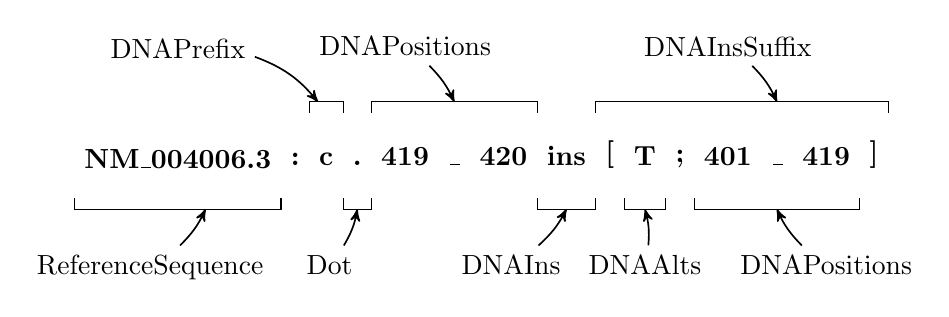
\begin{tikzpicture}[every edge/.append style={>=stealth',->,semithick}]
    \node at (0,0) [anchor=north west,rectangle,minimum height=1cm,text height=0.6cm]
      (refseq) {\bfseries NM\_004006.3};
    \node at (refseq.north east) [anchor=north west,rectangle,minimum height=1cm,text height=0.6cm,yshift=1]
      (colon) {\bfseries :};
    \node at (colon.north east) [anchor=north west,rectangle,minimum height=1cm,text height=0.6cm]
      (prefix) {\bfseries c};
    \node at (prefix.north east) [anchor=north west,rectangle,minimum height=1cm,text height=0.6cm]
      (dot) {\bfseries .};
    \node at (dot.north east) [anchor=north west,rectangle,minimum height=1cm,text height=0.6cm]
      (position1) {\bfseries 419};
    \node at (position1.north east) [anchor=north west,rectangle,minimum height=1cm,text height=0.6cm]
      (under1) {\bfseries \_};
    \node at (under1.north east) [anchor=north west,rectangle,minimum height=1cm,text height=0.6cm]
      (position2) {\bfseries 420};
    \node at (position2.north east) [anchor=north west,rectangle,minimum height=1cm,text height=0.6cm]
      (ins) {\bfseries ins};
    \node at (ins.north east) [anchor=north west,rectangle,minimum height=1cm,text height=0.6cm]
      (bracket1) {\bfseries [};
    \node at (bracket1.north east) [anchor=north west,rectangle,minimum height=1cm,text height=0.6cm]
      (T) {\bfseries T};
    \node at (T.north east) [anchor=north west,rectangle,minimum height=1cm,text height=0.6cm]
      (semicolon) {\bfseries ;};
    \node at (semicolon.north east) [anchor=north west,rectangle,minimum height=1cm,text height=0.6cm]
      (position3) {\bfseries 401};
    \node at (position3.north east) [anchor=north west,rectangle,minimum height=1cm,text height=0.6cm]
      (under2) {\bfseries \_};
    \node at (under2.north east) [anchor=north west,rectangle,minimum height=1cm,text height=0.6cm]
      (position4) {\bfseries 419};
    \node at (position4.north east) [anchor=north west,rectangle,minimum height=1cm,text height=0.6cm]
      (bracket2) {\bfseries ]};

    %\draw ([yshift=-36]refseq.south west) -- ([yshift=-40]refseq.south west)
    %   -- ([yshift=-39]bracket2.south east) -- ([yshift=-35]bracket2.south east);
    %  \node at (position2) [yshift=-60] {HGVS};

    \draw ([yshift=-5] refseq.south west) -- ([yshift=-9] refseq.south west)
      -- ([yshift=-9] refseq.south east) -- ([yshift=-5] refseq.south east);
      \node at ([xshift=-10,yshift=-30] refseq.south) {ReferenceSequence}
        edge[bend right=10] ([xshift=10,yshift=-9] refseq.south);

    %\draw ([yshift=2.5]prefix.south west) -- ([yshift=-1.5]prefix.south west)
    %  -- ([yshift=1]bracket2.south east) -- ([yshift=5]bracket2.south east);
    %  \node at (ins) [xshift=-10,yshift=-32] {Variant} edge[bend right=10] (bracket1.south);

    \draw ([yshift=-4] prefix.north west) -- (prefix.north west)
      -- (prefix.north east) -- ([yshift=-4] prefix.north east);
      \node at ([yshift=20]refseq.north) {DNAPrefix} edge[bend left=15] ([xshift=-3] prefix.north);

    \draw ([yshift=-6] dot.south west) -- ([yshift=-10] dot.south west)
      -- ([yshift=-10] dot.south east) -- ([yshift=-6] dot.south east);
      \node at ([xshift=-10,yshift=-30] dot.south) {Dot} edge[bend right=10] ([yshift=-10] dot.south);

    \draw ([yshift=-4] position1.north west) -- (position1.north west)
      -- (position2.north east) -- ([yshift=-4] position2.north east);
      \node at ([yshift=20]position1.north) {DNAPositions} edge[bend left=10] (under1.north);

    \draw ([yshift=-6] ins.south west) -- ([yshift=-10] ins.south west)
      -- ([yshift=-10] ins.south east) -- ([yshift=-6] ins.south east);
      \node at ([xshift=-20,yshift=-30] ins.south) {DNAIns} edge[bend right=10] ([yshift=-10] ins.south);

    \draw ([yshift=-4] bracket1.north west) -- (bracket1.north west)
      -- (bracket2.north east) -- ([yshift=-4] bracket2.north east);
      \node at ([yshift=20]position3.north) {DNAInsSuffix} edge[bend left=10] (under2.north);

    \draw ([yshift=-6] T.south west) -- ([yshift=-10] T.south west)
      -- ([yshift=-10] T.south east) -- ([yshift=-6] T.south east);
      \node at ([yshift=-30] T.south) {DNAAlts} edge[bend right=10] ([yshift=-10] T.south);

    \draw ([yshift=-6] position3.south west) -- ([yshift=-10] position3.south west)
      -- ([yshift=-10] position4.south east) -- ([yshift=-6] position4.south east);
      \node at ([yshift=-30] position4.south) {DNAPositions} edge[bend left=10] ([yshift=-10] under2.south);
\end{tikzpicture}
\end{frame}





\begin{frame}[plain]
\begin{figure}[!h]
  \centering
  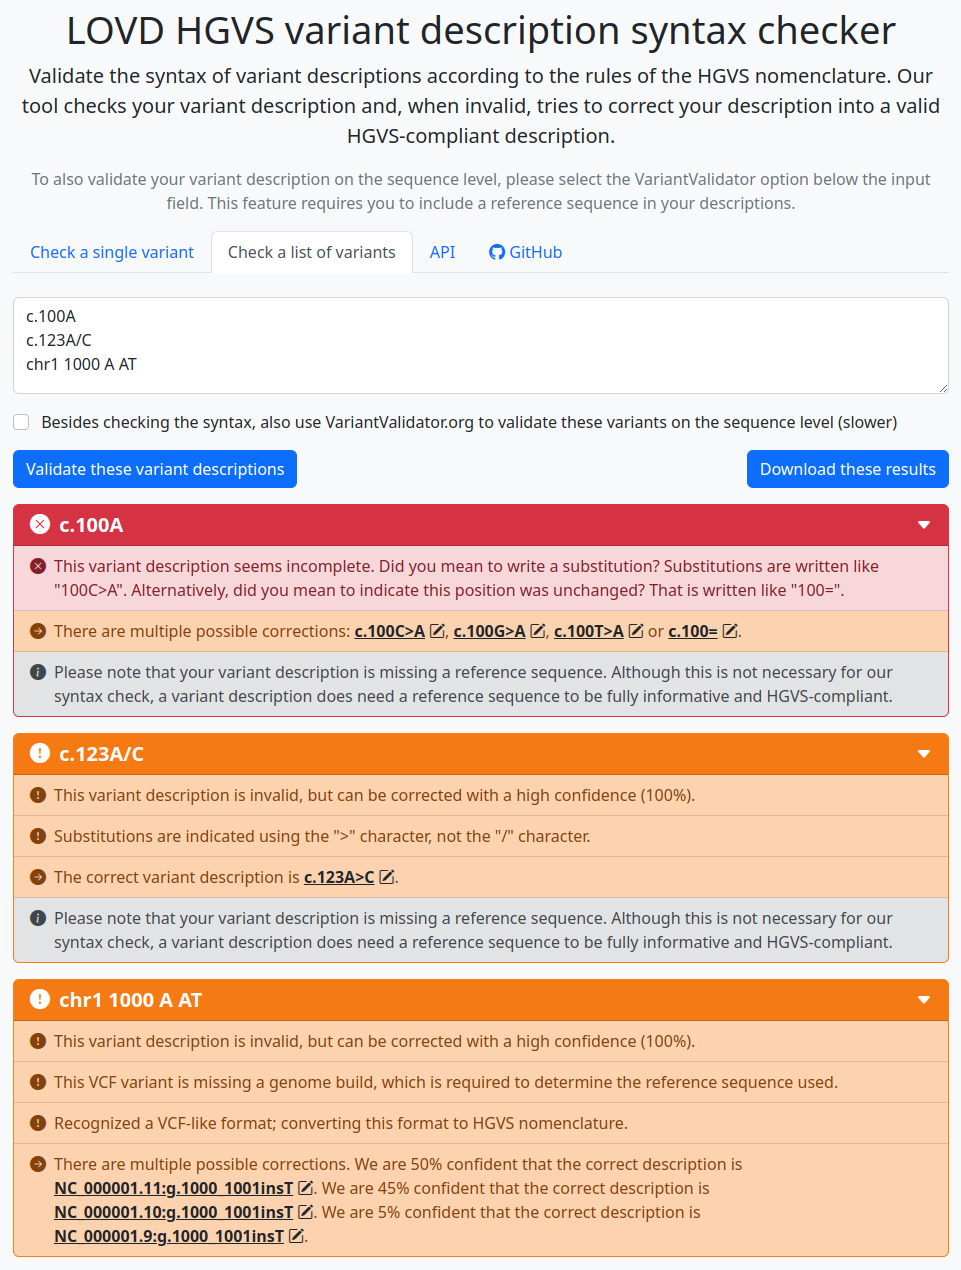
\includegraphics[height=\textheight]{figures_02.png}
\end{figure}
\end{frame}





\begin{frame}{Figure 3: Agreement with the HGVS nomenclature validation set.}
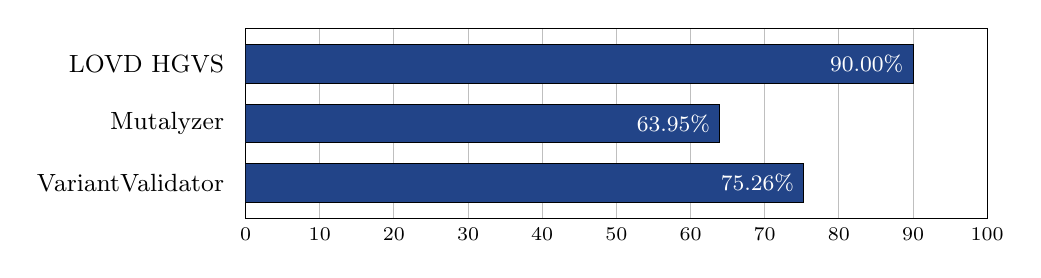
\begin{tikzpicture}
\begin{axis}[xbar,
  width=11cm,
  height=4cm,
  xmin=0,    % Don't let pgfplots scale the bars.
  xmax=100,  % Don't let pgfplots scale the bars.
  ymin=-3.6, % Don't let pgfplots scale the bars.
  ymax=-0.4, % Don't let pgfplots scale the bars.
  bar width={14pt},
  % Show measurements with the bars, and format.
  nodes near coords={\footnotesize\color{white}{\pgfmathprintnumber[fixed zerofill, precision=2]{\pgfplotspointmeta}\%}},
  nodes near coords align=left, % Measurements *in* the bar. {horizontal, left}
  % xlabel=\textbf{Title},
  xtick style={draw=none}, % Please don't draw the ticks.
  xticklabel style={font=\scriptsize},
  xmajorgrids=true,
  ytick={-1,...,-8}, % Easier to work with negatives, so the sorting of the graph works top to bottom.
  ytick style={draw=none}, % Please don't draw the ticks.
  yticklabels={LOVD HGVS, Mutalyzer, VariantValidator},
  yticklabel style={font=\small},
]
\addplot
[draw=black,fill=LOVD]
coordinates
{(90.00,-1) (63.95,-2) (75.26,-3)};
\end{axis}
\end{tikzpicture}
\end{frame}





\begin{frame}{Figure 4: Comparison of performance using the HGVS nomenclature validation set.}
\raggedleft
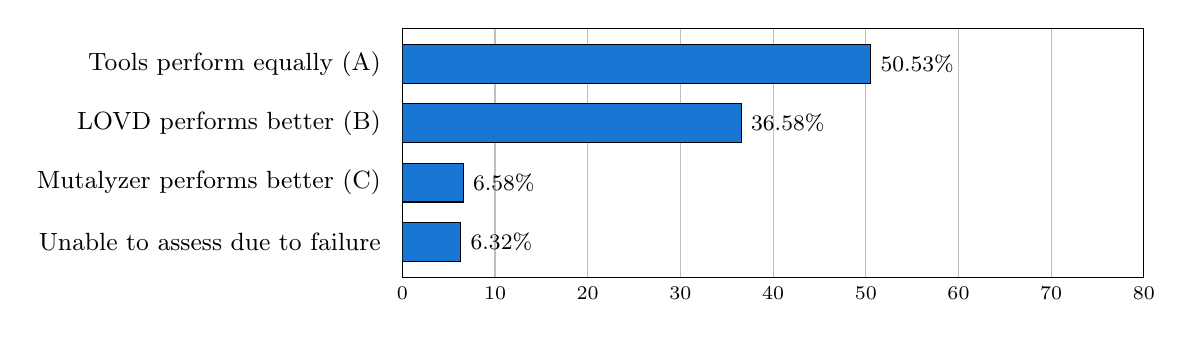
\begin{tikzpicture}
\begin{axis}[xbar,
  width=11cm,
  height=4.75cm,
  xmin=0,    % Don't let pgfplots scale the bars.
  xmax=80,   % Don't let pgfplots scale the bars.
  ymin=-4.6, % Don't let pgfplots scale the bars.
  ymax=-0.4, % Don't let pgfplots scale the bars.
  bar width={14pt},
  % Show measurements with the bars, and format.
  nodes near coords={\footnotesize\color{black}{\pgfmathprintnumber[fixed zerofill, precision=2]{\pgfplotspointmeta}\%}},
  %nodes near coords align=left, % Measurements *in* the bar. {horizontal, left}
  % xlabel=\textbf{Title},
  xtick style={draw=none}, % Please don't draw the ticks.
  xticklabel style={font=\scriptsize},
  xmajorgrids=true,
  ytick={-1,...,-8}, % Easier to work with negatives, so the sorting of the graph works top to bottom.
  ytick style={draw=none}, % Please don't draw the ticks.
  yticklabels={Tools perform equally (A), LOVD performs better (B),
    Mutalyzer performs better (C), Unable to assess due to failure},
  yticklabel style={font=\small},
]
\addplot
[draw=black,fill=Mutalyzer]
coordinates
{(50.53,-1) (36.58,-2) (6.32,-4) (6.58,-3)};
%Tools perform equally: 50.53%
%HGVS outperforms Mutalyzer: 36.58% (HGVS corrects more + HGVS handles more syntax + Mutalyzer is too tolerant + Mutalyzer normalization irregularity)
%Mutalyzer outperforms HGVS: 6.32% (HGVS is too tolerant + Mutalyzer corrects more + Mutalyzer handles more syntax)
%Unable to assess: 6.58%
\end{axis}
\end{tikzpicture}\hspace{5em}

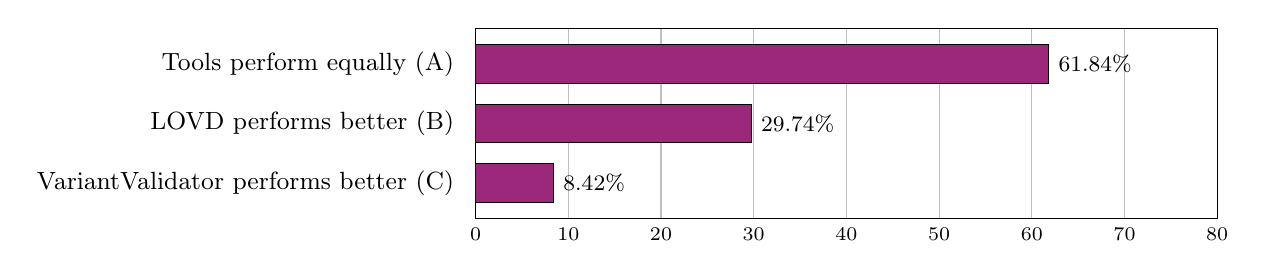
\begin{tikzpicture}
\begin{axis}[xbar,
  width=11cm,
  height=4cm,
  xmin=0,    % Don't let pgfplots scale the bars.
  xmax=80,   % Don't let pgfplots scale the bars.
  ymin=-3.6, % Don't let pgfplots scale the bars.
  ymax=-0.4, % Don't let pgfplots scale the bars.
  bar width={14pt},
  % Show measurements with the bars, and format.
  nodes near coords={\footnotesize\color{black}{\pgfmathprintnumber[fixed zerofill, precision=2]{\pgfplotspointmeta}\%}},
  %nodes near coords align=left, % Measurements *in* the bar. {horizontal, left}
  % xlabel=\textbf{Title},
  xtick style={draw=none}, % Please don't draw the ticks.
  xticklabel style={font=\scriptsize},
  xmajorgrids=true,
  ytick={-1,...,-8}, % Easier to work with negatives, so the sorting of the graph works top to bottom.
  ytick style={draw=none}, % Please don't draw the ticks.
  yticklabels={Tools perform equally (A), LOVD performs better (B), VariantValidator performs better (C)},
  yticklabel style={font=\small},
]
\addplot
[draw=black,fill=VV]
coordinates
{(61.84,-1) (29.74,-2) (8.42,-3)};
%Tools perform equally: 61.84%
%HGVS outperforms VV: 29.74% (HGVS corrects more + HGVS handles more syntax + VV is too tolerant + VV normalization irregularity)
%VV outperforms HGVS: 8.42% (HGVS is too tolerant + VV corrects more + VV handles more syntax)
\end{axis}
\end{tikzpicture}\hspace{5em}

\end{frame}
\end{document}%%%%%%%%%%%%%%%%%%%%%%%%%%%%%%%%%%%%%%%%%%%%%%%%%%%%%%%%%%%%%%%%%%%%%%%%%%%%%%%%%%%%%%%%%%%%%%%%%%%%%%%%%%
